

\documentclass[10pt]{extarticle}

\usepackage[utf8]{inputenc}
\usepackage{extsizes} % Allow for more sizes such as 14pt or 17pt on document class.
\usepackage{mathtools} % Allows conditional math expressions, etc.

% Don't output references in case they're empty - http://tex.stackexchange.com/questions/74476/how-to-avoid-empty-thebibliography-environment-bibtex-if-there-are-no-refere

\let\myBib\thebibliography
\let\endmyBib\endthebibliography

\renewcommand\thebibliography[1]{\ifx\relax#1\relax\else\myBib{#1}\fi}


\begin{document} 



%% Front page.
\title{07.01 - Support Vector Machines}

    
    \date{}
    

    

    \maketitle

\newpage
%% Abstract page.


%% Table of contents page.



%% Body start.
\section{Optimization objective}\label{optimization-objective}

In support vector machine, we don't directly have $\lambda$. Instead, C
is used, which penalizes the training set instead of the $\theta$. In
reality, it's almost the same, as we can set a small value for C and
then we're giving more importance to the regularization term. We could
think of $C = \frac{1}{\lambda}$.

A part from that, the objective function (minimizing cost function) is
almost the same as the logistic regression one:

\begin{equation} 
min_{\theta} C \sum_{i=1}^m [y^{(i)}cost_1(\theta^T x^{(i)}) + (1 - y^{(i)})cost_0(\theta^T x^{(i)})] + \frac{1}{2} \sum_{j=1}^n \theta_j^2
\end{equation}

Where $cost_0$ and $cost_1$ are functions that are applied when $y = 0$
and $y = 1$, respectively. \smallskip

SVMs don't output probabilities, they output directly the class they
classificate into, using the following hyphotesis:

\begin{equation} 
h_\theta(x) = 
\begin{dcases}
    1, & \text{if\,} \theta^Tx \geq 0 \\ 
    0, & \text{otherwise}
\end{dcases} 
\end{equation}

\section{Large Margin Intuition}\label{large-margin-intuition}

We can see the SVM as a large margin classifier, meaning that if we have
linearly separable data, it will separate it optimizing the boundary
distance between the data (fig \ref{fig:large_margin}).

\begin{figure}
\centering
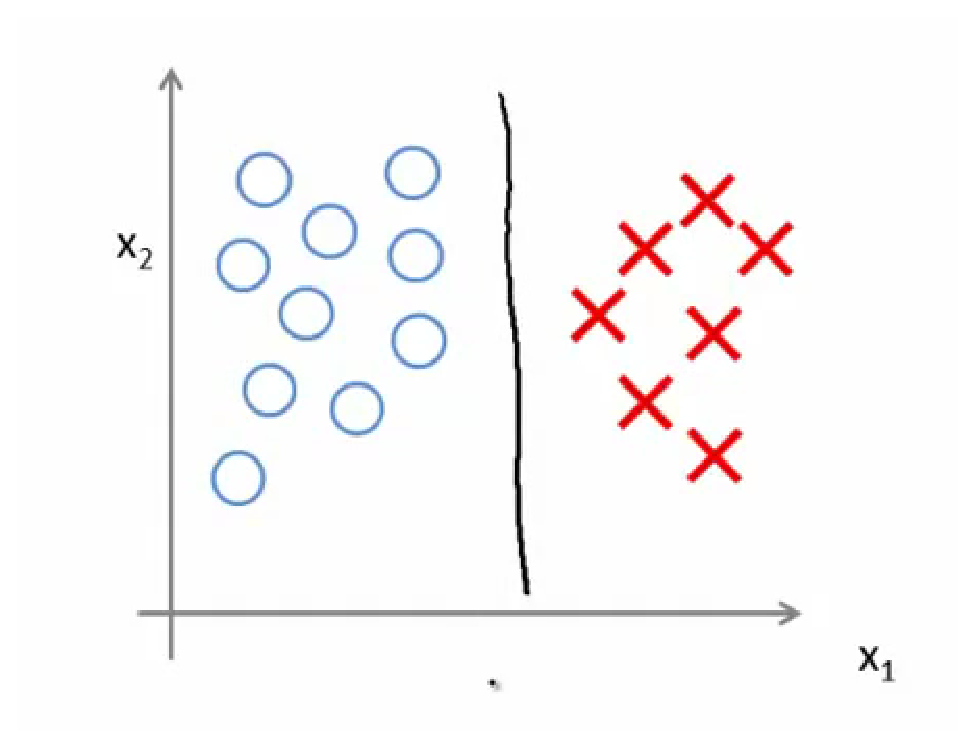
\includegraphics[width=\textwidth]{img/large_margin.eps}
\caption{Example of linearly separable data correctly classified by an SVM.}
\label{fig:large_margin}
\end{figure}

\section{Kernels I}\label{kernels-i}

In logistic regression, when we had a non-linear problem, we had to use
polynomial features. Kernels are another way of getting more features
out of the training sample. \smallskip

Kernels are similarity functions. In the video, he selects 3 landmarks
and uses a gaussian kernel. He then uses those 3 landmarks to compute 3
features, using the gaussian to know the similarity between x and each
of the landmark.

Doing that, we can create a decision boundary around the landmarks,
where everything near them gets classified as 1 and everything that is
far from them gets classified as 0 (following a gaussian shape).

\section{Kernels II}\label{kernels-ii}

\subsection{Choosing Landmarks}\label{choosing-landmarks}

For every training example, get a landmark exactly at that location.
Then, features will be based around the similarity of a point in our
data to other points. This way we have one feature per datapoint, so we
have m features. \smallskip

Basically, we just substitute the features we had and we use this ones.

Mathematical implemenation note:

\begin{equation} 
\sum_{j=1}^n \theta_j^2 = \theta^t M \theta
\end{equation}

Where M is a matrix that depends on the kernel. This is done to scale to
bigger training sets.

\subsection{SVM Parameters}\label{svm-parameters}

\begin{itemize}
\itemsep1pt\parskip0pt\parsep0pt
\item
  Large C: Lower bias, high variance (small $\lambda$).
\item
  Small C: Higher bias, low variance (large $\lambda$).
\end{itemize}

\section{Using an SVM}\label{using-an-svm}

\begin{itemize}
\itemsep1pt\parskip0pt\parsep0pt
\item
  Use SVM software package to solve for paraemters $\theta$.
\item
  You still need to specify the choice of parameter C and the kernel.
\item
  No kernel is sometimes called ``linear kernel''.
\item
  Do perfrom feature scaling before using the kernel.
\end{itemize}

Not all similarity functions make valid kernels. They need to satisfy a
technical condition called ``Mercer's Theorem''.

\subsection{Multiclass classification}\label{multiclass-classification}

Many SVM packages already have built-in multi-class classification
functionality. Otherwise, use one-vs-all.

\subsection{Logistic regression vs
SVMs}\label{logistic-regression-vs-svms}

Let n = number of features and m = number of training examples.
\smallskip

\begin{itemize}
\itemsep1pt\parskip0pt\parsep0pt
\item
  If n is large relative to m -\textgreater{} Use logistic regression or
  SVM without kernel.
\item
  If n is small, m is intermediate -\textgreater{} Use SVM with Gaussian
  kernel.
\item
  If n is small, m is large -\textgreater{} Create/Add features and then
  use logistic regression or SVM without kernel.
\end{itemize}

Neural networks is likely to work well for mos of these settings, but
they're way slower to train.

SVMs don't have to worry about local optima, because they solve a convex
problem. NN may have problems with that, though.


%% Body end.

%% Bibliography.

    \nocite{*}

\bibliographystyle{plain}
\bibliography{references}

\end{document}